\chapter{The basics of designing, compiling and executing programming languages}

% theoretische methodischen Grundlagen, die im weiteren Verlauf bei der Problemlösung im praktischen Teil eine wichtige Rolle spielen
% Detailgrad so hoch, wie für Verständnis nötig (Leser ist anonymer Informatiker)
% >= 25%

    \section{Designing programming languages}
    
    	%TODO
    	\todo[inline]{To what degree do I need references here?}
		
		There are many different kinds of programming languages. They can vary in many aspects, from the general approach to small details. What are some important aspects?
		
		%\subsection{Domain}
		%simplicity and power
		Firstly there's the matter of what the language is trying to achieve. Is it supposed to be a generalist programming language, suitable for writing any kind of software? Or is it a domain specific language, built to solve a specific problem elegantly? In the latter case, the language will likely be a lot simpler due to its reduced scope.
		
		\subsection{Programming paradigms}
		Then there are different approaches to programming -- programming paradigms. The reader is likely familiar with imperative programming, which describes programs in terms of statements being executed to change state, and object-oriented programming, which models problems as interacting objects consisting of data and methods of working with it. Another example is functional programming, which includes no mutable state and where the results of functions are purely defined in terms of their parameters, and there are numerous other paradigms. A programming language may only follow one or be multi-paradigm, mixing them.
		
		\subsection{Type system}
		%static vs dynamic typing
		Its type system is another important aspect of a programming language, and an essential characteristic of a type system is whether it has dynamic or static typing: Values have a type, for example integral, boolean or array types. In static typing these types are resolved at compile time; variables and parameters have a well-defined type, either explicitly stated or inferred, and trying to use a value of incompatible type results in a compile error.
		%TODO mention how that encourages complex type systems?
		Dynamic type systems annotate values with their type at run time, and only then do type errors occur. This can make it easier to write generic code, but mistakes also go unnoticed more easily with the decrease in compile time errors.
		
		In some programming languages variables, which can usually change their value, can be marked as immutable -- or constant, as it is sometimes called in this context. The value of these variables may no longer be changed after their initial assignment. This allows for better expression of intent, preventing accidental misuse. One useful application for this is marking by-reference parameters as read-only.
		
		%TODO phrasing?
		Another concept is that of a pure function, which is one whose output depends solely on its parameters and which has no side effects. So it doesn't depend on any global state and doesn't change it. This makes it easier to reason about and test since it will always behave the same way given the same parameters. Some functional languages require all functions to be pure, while some other languages let the programmer explicitly mark the function as pure/impure, again preventing them from taking unintended actions.
		
		\subsection{Coroutines}
		
		A coroutine is a strand of execution with its own (call) stack. When the program starts, there's a single coroutine starting execution at the entry point. This coroutine may then launch new coroutines, at which point its execution is halted and the new coroutine starts its execution. They don't run in parallel, there's exactly one active coroutine (per thread) at any point. Only when this new coroutine stops its execution -- either permanently, by returning, or temporarily, by yielding; in either case a value may be passed back to the previous coroutine -- does the previous one resume its execution. A paused coroutine -- one that yielded -- may later be resumed, possibly passing in a new value.
		
		One example where coroutines are useful is iterating through recursive data structures like a binary tree. A coroutine can recurse through the tree, yielding every node it visits, which to the caller of the coroutine looks much like a function that yields the next node each time it's called.
		
		\begin{codelisting}[caption={Pseudocode of tree iteration using coroutines}]
function yield_nodes( tree ):
    if tree:
        yield tree.value
        yield_nodes( tree.left_subtree )
        yield_nodes( tree.right_subtree )

function print_nodes( tree ):
    for node in yield_nodes( tree ):
        print( node )
		\end{codelisting}
	
	\section{Compilers}
	
		\todo[inline]{This chapter needs references.}
	
		Compilers translate one language -- the source language -- to another -- the target language. The Java compiler for example translates Java source code to Java Byte Code. This translation consists of multiple steps: First the input, which is essentially treated as a long sentence, is split into tokens, which can be thought of as words, by the lexer. The parser then performs a syntactical analysis on these words, creating a syntax tree. Semantic analysis then verifies this tree makes sense: Where are the referenced variables and functions? In the case of statically typed languages, do the types match? During this process, the syntax tree may be transformed and annotated it with additional information. Next, optimization may take place, transforming the syntax tree into an equivalent but in some way better version, before finally the target code is generated.

		\subsection{Chomsky hierarchy}
			
			Formal languages can be derived from formal grammars, and the Chomsky hierarchy ranks these grammars by how difficult they are to parse, with Type-0 grammars being the most difficult and Type-3 grammars the easiest. Of particular interest for compiler construction are the two easiest types, Type-3 and Type-2 grammars.
			
			\subsubsection{Regular languages}
			
			Type-3 grammars describe regular languages and can be expressed as regular expressions. Regular expressions consist of terminal symbols -- characters in the alphabet of the language -- and operations combining them, as well as $\epsilon$, the empty word, which is not usually explicitly used outside of formal definitions but implied in absence of a character. These are the core operations:
			
			 %The first operation is concatenation, and is simply written as such: $ab$ means expression $a$ followed by expression $b$. The alternative operator $|$ is usually understood to have a lower precedence than concatenation, so $ab|cd$ means $(ab)|(cd)$ and explicit parentheses are required if the intended meaning is $a(b|c)d$. The operation with the highest precedence is the unary Kleene star, which is defined as any number of concatenations, including none, i.e. the empty word; it's written as $a*$, which 
			
			\begin{center}
			\begin{tabular}{ l l p{10cm} }
			\toprule
			Name         & Syntax & Description \\
			\midrule
			Concatenation & $ab$  & Expression $a$ followed by expression $b$. \\
			Alternative   & $a|b$ & Either expression $a$ or expression $b$; lower precedence than concatenation, so $ab|cd$ means $(ab)|(cd)$ and explicit parentheses are required if $a(b|c)d$ is the intention. \\
			Kleene Star   & $a*$  & Any number of repetitions of expression $a$, including none, i.e. $\epsilon|a|aa|aaa|\ldots$; highest precedence, so $ab*c$ means $a(b*)c$. \\
			\bottomrule
			\end{tabular}
			\end{center}
			
			Some auxiliary operators are often defined in terms of them, like $a+ = aa*$ and $a? = a|\epsilon$, but those are merely substitutions, they don't add any capabilities, and thus don't require further investigation.
			
			%TODO
			\todo[inline]{I suppose I should mention [a-z]-style character classes at some point?}
			
			Regular languages can be recognized by finite automatons. There are two kinds of finite automatons: deterministic and non-deterministic finite automatons. The more practical one to build is the deterministic finite automaton (DFA). It has a finite set of states, one of which is the start state and some of which are accept states, an input alphabet and a transition function which defines the resulting state for each pair of current state and input character. Initially, the automaton is in its start state; the input is then processed one character at a time: the current state changes according to the transition function given the current input character, until all input characters have been processed and a certain state has been reached. If this state is an accept state, the input is accepted, i.e. it is part of the regular language.
			
			The transition function can be partial; if it is not defined for a given state-character-pair, the input is not accepted. This simplifies its definition. If a total definition is preferred, a fail-state to which all formerly undefined transitions lead can be introduced.
			
			Non-deterministic finite automatons (NFAs) are mostly the same, only the transition function works differently: Firstly, it does not define a single resulting state for any given input, but a set of possible resulting states, any of which may be entered. Secondly, it is not just defined for input characters, but also $\epsilon$ inputs, i.e. spontaneous $\epsilon$-transitions that consume no input are possible. An input is thus considered accepted if its processing \textit{may} end in an accept state. Due to their non-deterministic nature DFAs are impractical to build, but as an intermediate model they are useful, as will become apparent shortly.
			
			Finite automatons can be represented as directed graphs, with states being the nodes and transitions being the edges, annotated with the input. By convention, accept states are encircled and the start state is indicated by an arrow pointing to it. This notation will be used frequently throughout this chapter due to its simplicity and brevity.
			
			NFAs are so useful in the context of compilers because regular expressions can be directly translated to them. Only a handful of rules have to be applied recursively, as outlined in figures \ref{fig:re_nfa_char}--\ref{fig:re_nfa_kleene}\footnote{To understand the need for states 1 and 4 in figure \ref{fig:re_nfa_kleene} think about the translation of $a*b*$.}. A simple example of this is given in figure \ref{fig:re_nfa_example}.
			
			
			\begin{figure}
			\centering
			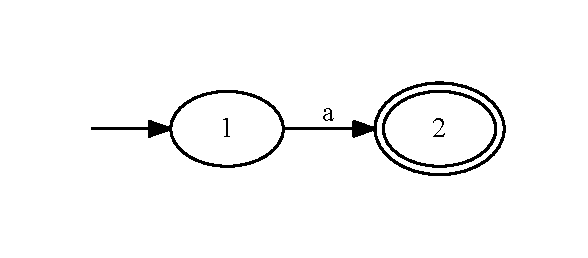
\includegraphics{figures/re_char}
			\caption{NFA for the regular expression ``$a$'' -- i.e. a single character}
			\label{fig:re_nfa_char}
			\end{figure}
			
			\begin{figure}
			\centering
			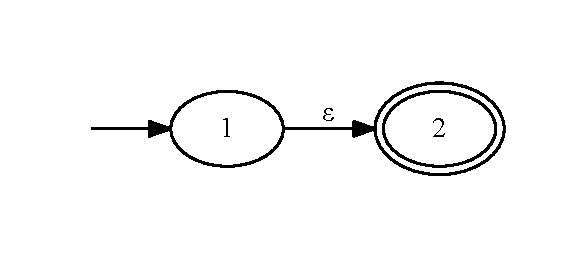
\includegraphics{figures/re_epsilon}
			\caption{NFA for the regular expression ``'' -- i.e. the empty string}
			\label{fig:re_nfa_epsilon}
			\end{figure}
			
			\begin{figure}
			\centering
			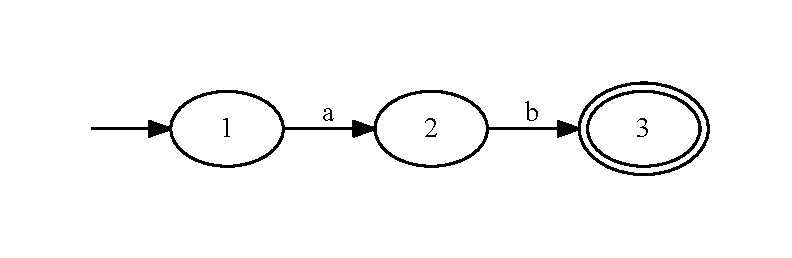
\includegraphics{figures/re_sequence}
			\caption{NFA for the regular expression ``$ab$'' -- i.e. a concatenation}
			\label{fig:re_nfa_concatenation}
			\end{figure}
			
			\begin{figure}
			\centering
			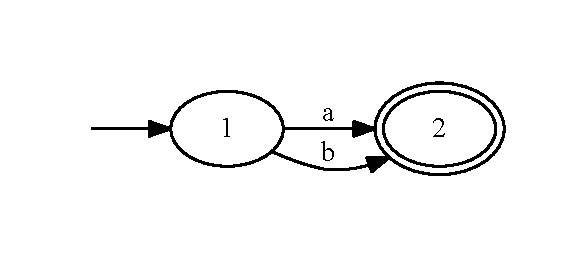
\includegraphics{figures/re_alternative}
			\caption{NFA for the regular expression ``$a|b$'' -- i.e. an alternative}
			\label{fig:re_nfa_alternative}
			\end{figure}
			
			\begin{figure}
			\centering
			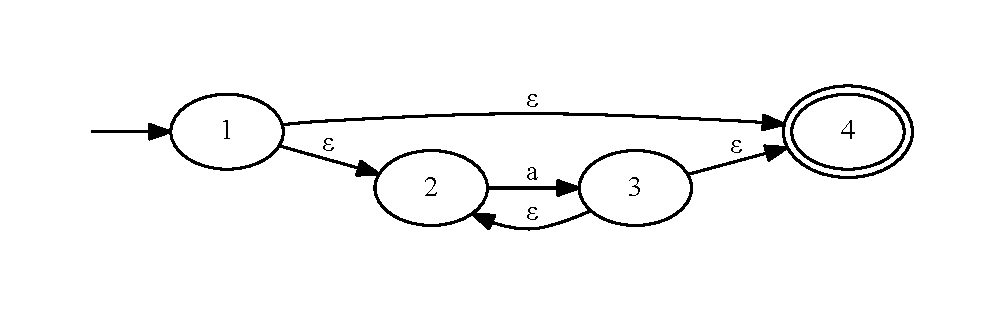
\includegraphics[width=\textwidth]{figures/re_kleene}
			\caption{NFA for the regular expression ``$a*$'' -- i.e. a repetition}
			\label{fig:re_nfa_kleene}
			\end{figure}
			
			\begin{figure}
			\centering
			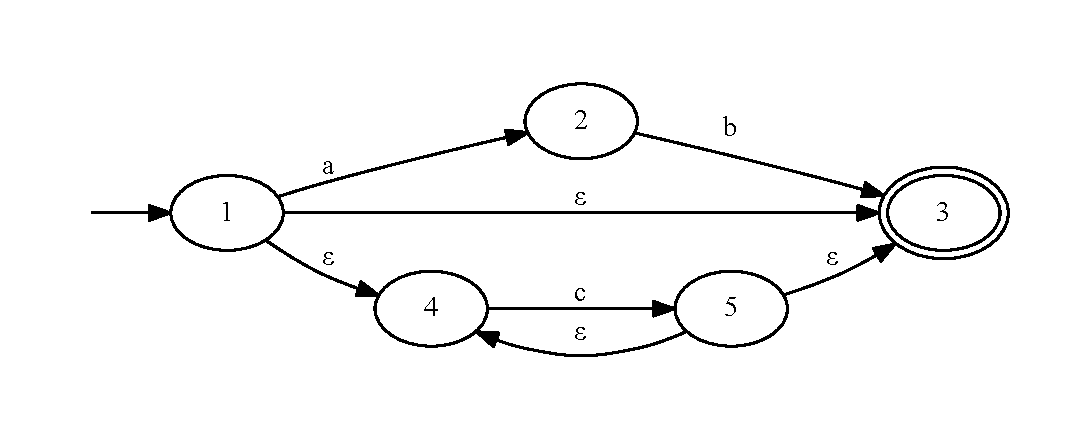
\includegraphics[width=\textwidth]{figures/re_example}
			\caption{NFA for the regular expression ``$ab|c*$''}
			\label{fig:re_nfa_example}
			\end{figure}
			
			NFAs may be impractical to build, but any NFA can be converted into a (practical) DFA accepting the same language. This DFA has as its states sets of states from the NFA: The initial state is the set containing the NFA's initial state and any state reachable from it using $\epsilon$-transitions. For each character there's a transition to the set of NFA states reachable from any of the states in the previous set using this character and any number of $\epsilon$-transitions. Accept states are all sets containing NFA accept states.
			
			By way of an example, figure \ref{fig:re_dfa_example} shows the DFA equivalent of the NFA in figure \ref{fig:re_nfa_example}.
			
			\begin{figure}
			\centering
			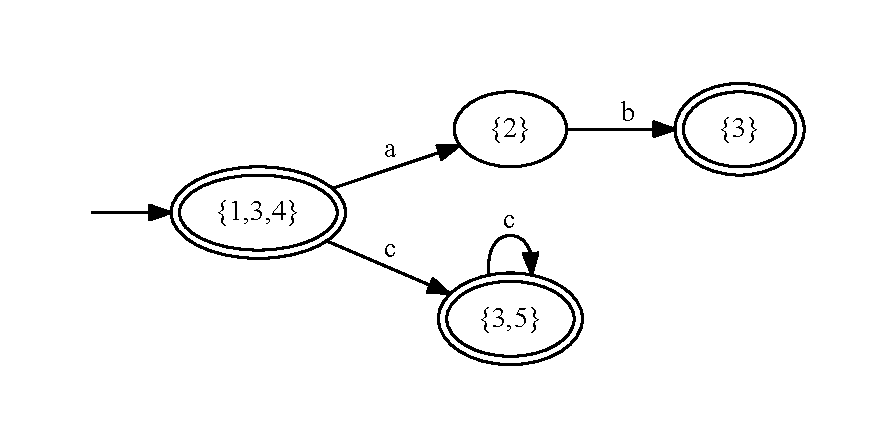
\includegraphics[width=\textwidth]{figures/re_example_dfa}
			\caption{DFA equivalent of the NFA in figure \ref{fig:re_nfa_example}}
			\label{fig:re_dfa_example}
			\end{figure}
			
			\subsubsection{Context-free languages}
		
		\subsection{Lexer}
		
		\subsection{Parser}
			
			LL, (LA)LR, GLR, ...
			
		\subsection{Semantic Analysis}
		
		\subsection{Optimization}
		
			tail calls?
		
		\subsection{Code generation}

	\section{Virtual Machines}
	
		VM vs Native code
		
		\subsection{Details} % TODO: name
			fetch \& execute
			
			stack based vs registers
			
			garbage collection
			
			opcodes \& choosing them
			
			error handling
			
			stack unwinding?
	
	\section{Relevant software patterns and language features}
	
		RAII
		
		Sum Types
		
		Optional
		
		Iterators
		
		Visitor
		
		Templates
		
		(Macros)
		
		Operator overloading
		
		Serialization
